\coursefooterdate{?.06.2024}
\head{\Large Урок 4: Шаблоны, наследование и структуры на основе Vector.}
\label{md2tex4}
\hyperref[md2texREADME]{К главному описанию}


\subhead{Краткий план}
\begin{enumerate}
    \item Зачем нужны шаблоны и как они разбиваются на файлы.
    \item Stack на основе Vector: наследование.
    \item Queue с помощью двух Stack как полей класса.
\end{enumerate}


\subhead{Мотивация}
Вроде бы мы справились сделать Vector, хранящий int. А что если нам понадобится хранить string, float, double, long long, char - под всё это заново класс писать что-ли?! К счастью нет, и в C++ для этих целей придуманы шаблоны.


\subhead{Как работать с шаблонами}
В объявлении класс (\mintinline{cpp}{.h} файл) сразу над классом добавляем и над функцией вывода:
\begin{minted}{cpp}
template<typename T>
\end{minted}
И внутри объявления класс меняем используем \mintinline{cpp}{T} как тип, хранимый в векторе.

В реализации класса (\mintinline{cpp}{.cpp} файл) перед каждым методом нужно добавить:
\begin{minted}{cpp}
template<typename T>
\end{minted}
И заменить \mintinline{cpp}{Vector} на \mintinline{cpp}{Vector<T>} везде, где имеется ввиду тип данных (то есть все места, кроме названия конструктора и деструктора).

И наконец переименовываем \mintinline{cpp}{vector.cpp} в \mintinline{cpp}{vector.tpp} и добавляем в конце \mintinline{cpp}{vector.h} строку:
\begin{minted}{cpp}
#include "vector.tpp"
\end{minted}
Подключать файл в заголовочный нужно так как шаблонный класс должен подключаться в другие файлы целиком (вместе с реализацией всех методов), а поменяли расширение мы для того, чтобы отличать файл с настоящим кодом от файла с шаблоном кода (у MSWord сделано также: для обычных файлов и файлов с шаблоном стиле используются разные расширения).


\subhead{Стек}
Стек - это такая структура данных, которая позволяет только добавлять и удалять элемент из конца, обращаться к последнему элементу. По сути это только часть функционала, которую мы уже сделали в Vector, и зачем мы вообще останавливаемся на стеке? Это может показаться странным, но на практике люди любят искусственно ограничить себе возможности: если вы хотите использовать только функционал стека, то хочется использовать отдельный класс для стека, а не использовать вектор - так код упрощается для чтения и потенциально может стать эффективнее от использования структуры данных умеющей меньше. Но хоть структура и простая, но мы постараемся максимально усложнить себе жизнь!

Мы уже познакомились с инкапсуляцией, когда рассматривали модификаторы доступа. Теперь настало время рассмотреть наследование. Представим, что мы хотим в классе \mintinline{cpp}{Child} сделать примерно тоже самое, что делали в классе \mintinline{cpp}{Parent} но с какими-то отличиями. Тогда мы можем унаследовать \mintinline{cpp}{Child} от \mintinline{cpp}{Parent} и поменять только нужные функции. Это хорошая практика, так как позволяет уменьшить объём кода в отличие от полного копирования всех методов. В C++ придумали несколько видов наследования:
\begin{minted}{cpp}
class Child : public Parent;
class Child : protected Parent;
class Child : private Parent;
\end{minted}
Если не указать модификатор, то по умолчанию используется \mintinline{cpp}{private} (а для \mintinline{cpp}{struct} используется \mintinline{cpp}{public}). Общая схема того, как наследуются поля:

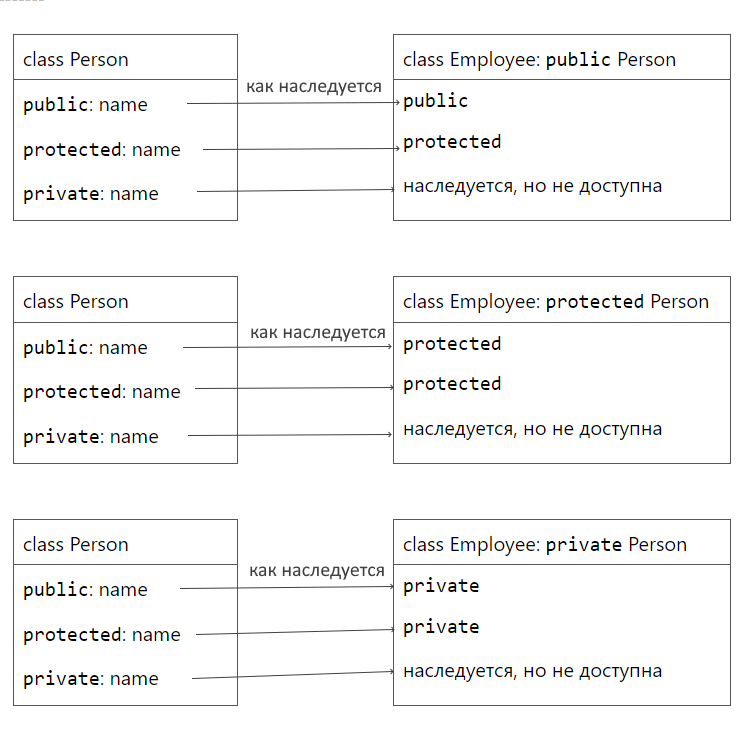
\includegraphics[scale=0.4]{lessons/4-inheritance.png}

Когда в \mintinline{cpp}{Child} мы хотим использовать метод \mintinline{cpp}{method} унаследованный из \mintinline{cpp}{Parent}, то его можно вызвать через \mintinline{cpp}{Parent::method}.

Для стека мы хотим приватно унаследоваться от вектора и переименовать методы в \mintinline{cpp}{push}, \mintinline{cpp}{top}, \mintinline{cpp}{pop}. Деструктор у нас ничего делать не будет, так как C++ сам вызывает деструктор родительского класса. Обращение по индексу, методы \mintinline{cpp}{begin} и \mintinline{cpp}{end}, операцию вывода тоже можно определить, но они не очень осмысленны к структуре с возможностью доступа только к последнему элементу.

Ещё из приятных фактов стоит отметить, что конструктор копирования и оператор присваивания можно определять, а довериться в их создании компилятору. Компилятор справляется сам сгенерировать эти методы, если в самом классе не хранится что-то сложное (в нашем случе в Vector хранилась \mintinline{cpp}{data} и мы следили чтобы она правильно копировалась, в Stack же ничего не хранится и компилятор сгенерирует функции через копирования в Vector).

Но если очень хочется, то можно определить конструктор и вызывать в нём родительский конструктор, например вот такой код допустим:
\begin{minted}{cpp}
template<typename T>
Stack<T>::Stack() : Vector<T>::Vector() {}      // Вызываем родительский конструктор без аргументов
\end{minted}


\subhead{Очередь}
Теперь мы перейдём к такой структуре, как очередь (Queue). Функционал у очереди тоже довольно маленький: можно добавить элемент в конец и взять из начала. И очередь можно реализовать с помощью двух стеков \mintinline{cpp}{left} и \mintinline{cpp}{right}
\begin{itemize}
    \item При добавлении элемента добавляем его в \mintinline{cpp}{right}.
    \item Если мы удаляем элемент и \mintinline{cpp}{left} пустой, то перекладываем все элементы из \mintinline{cpp}{right} в \mintinline{cpp}{left} и переходим к следующему шагу.
    \item Если мы удаляем элемент и \mintinline{cpp}{left} не пустой, то удаляем из \mintinline{cpp}{left}.
\end{itemize}

Понятно, что очередь не нужно не от чего наследовать, так как левая и правая части достаточно равнозначны. Поэтому в очереди будем хранить два стека. Все методы определяются по описанию выше, разве что вынести перекладывание всех элементов из \mintinline{cpp}{right} в \mintinline{cpp}{left} можно в отдельную функцию \mintinline{cpp}{move_stack} (она должна быть \mintinline{cpp}{private}), чтобы кто попало её не вызывал.

Кроме того стоит отметить, что метод \mintinline{cpp}{front} пришлось сделать неконстантным, так как если \mintinline{cpp}{left} пуст, то мы не можем достать элемент снизу \mintinline{cpp}{right}. В целом это можно обойти, если никогда не оставлять \mintinline{cpp}{left} пустым, или добавить метод в стек. То есть ограничения на некоторые методы бывают вызваны внутренним устройством структуры и это нормально.
